\documentclass[12pt,a4paper]{article}
\usepackage[utf8]{inputenc}
\usepackage[T1]{fontenc}
\usepackage{fontspec}
\usepackage[polish]{babel}
\usepackage{amsmath}
\usepackage{graphicx}
\usepackage[table,xcdraw]{xcolor}
\usepackage{hhline}
\usepackage{placeins}
\usepackage[margin=0.6in]{geometry}
\usepackage{appendix}
\usepackage{colortbl}
\usepackage{physics}
\usepackage{float}
\usepackage{datetime}
\usepackage{hyperref}

\title{Praca Domowa Termodynamika i Fizyka Statystyczna R 2021/2022}
\author{Kacper Cybiński}
% \newdate{date}{28}{01}{2022}
% \date{\displaydate{date}}
\date{\today}
\setlength\parindent{0pt}

\newcommand{\com}[1]{{\color{red} #1}}

\newcommand{\link}[2]{{\color{cyan} \href{#1}{#2}}}

\renewcommand{\emph}{\textbf}

\begin{document}

\maketitle

\section{Zadanie 1s}

\begin{figure}[h!]
    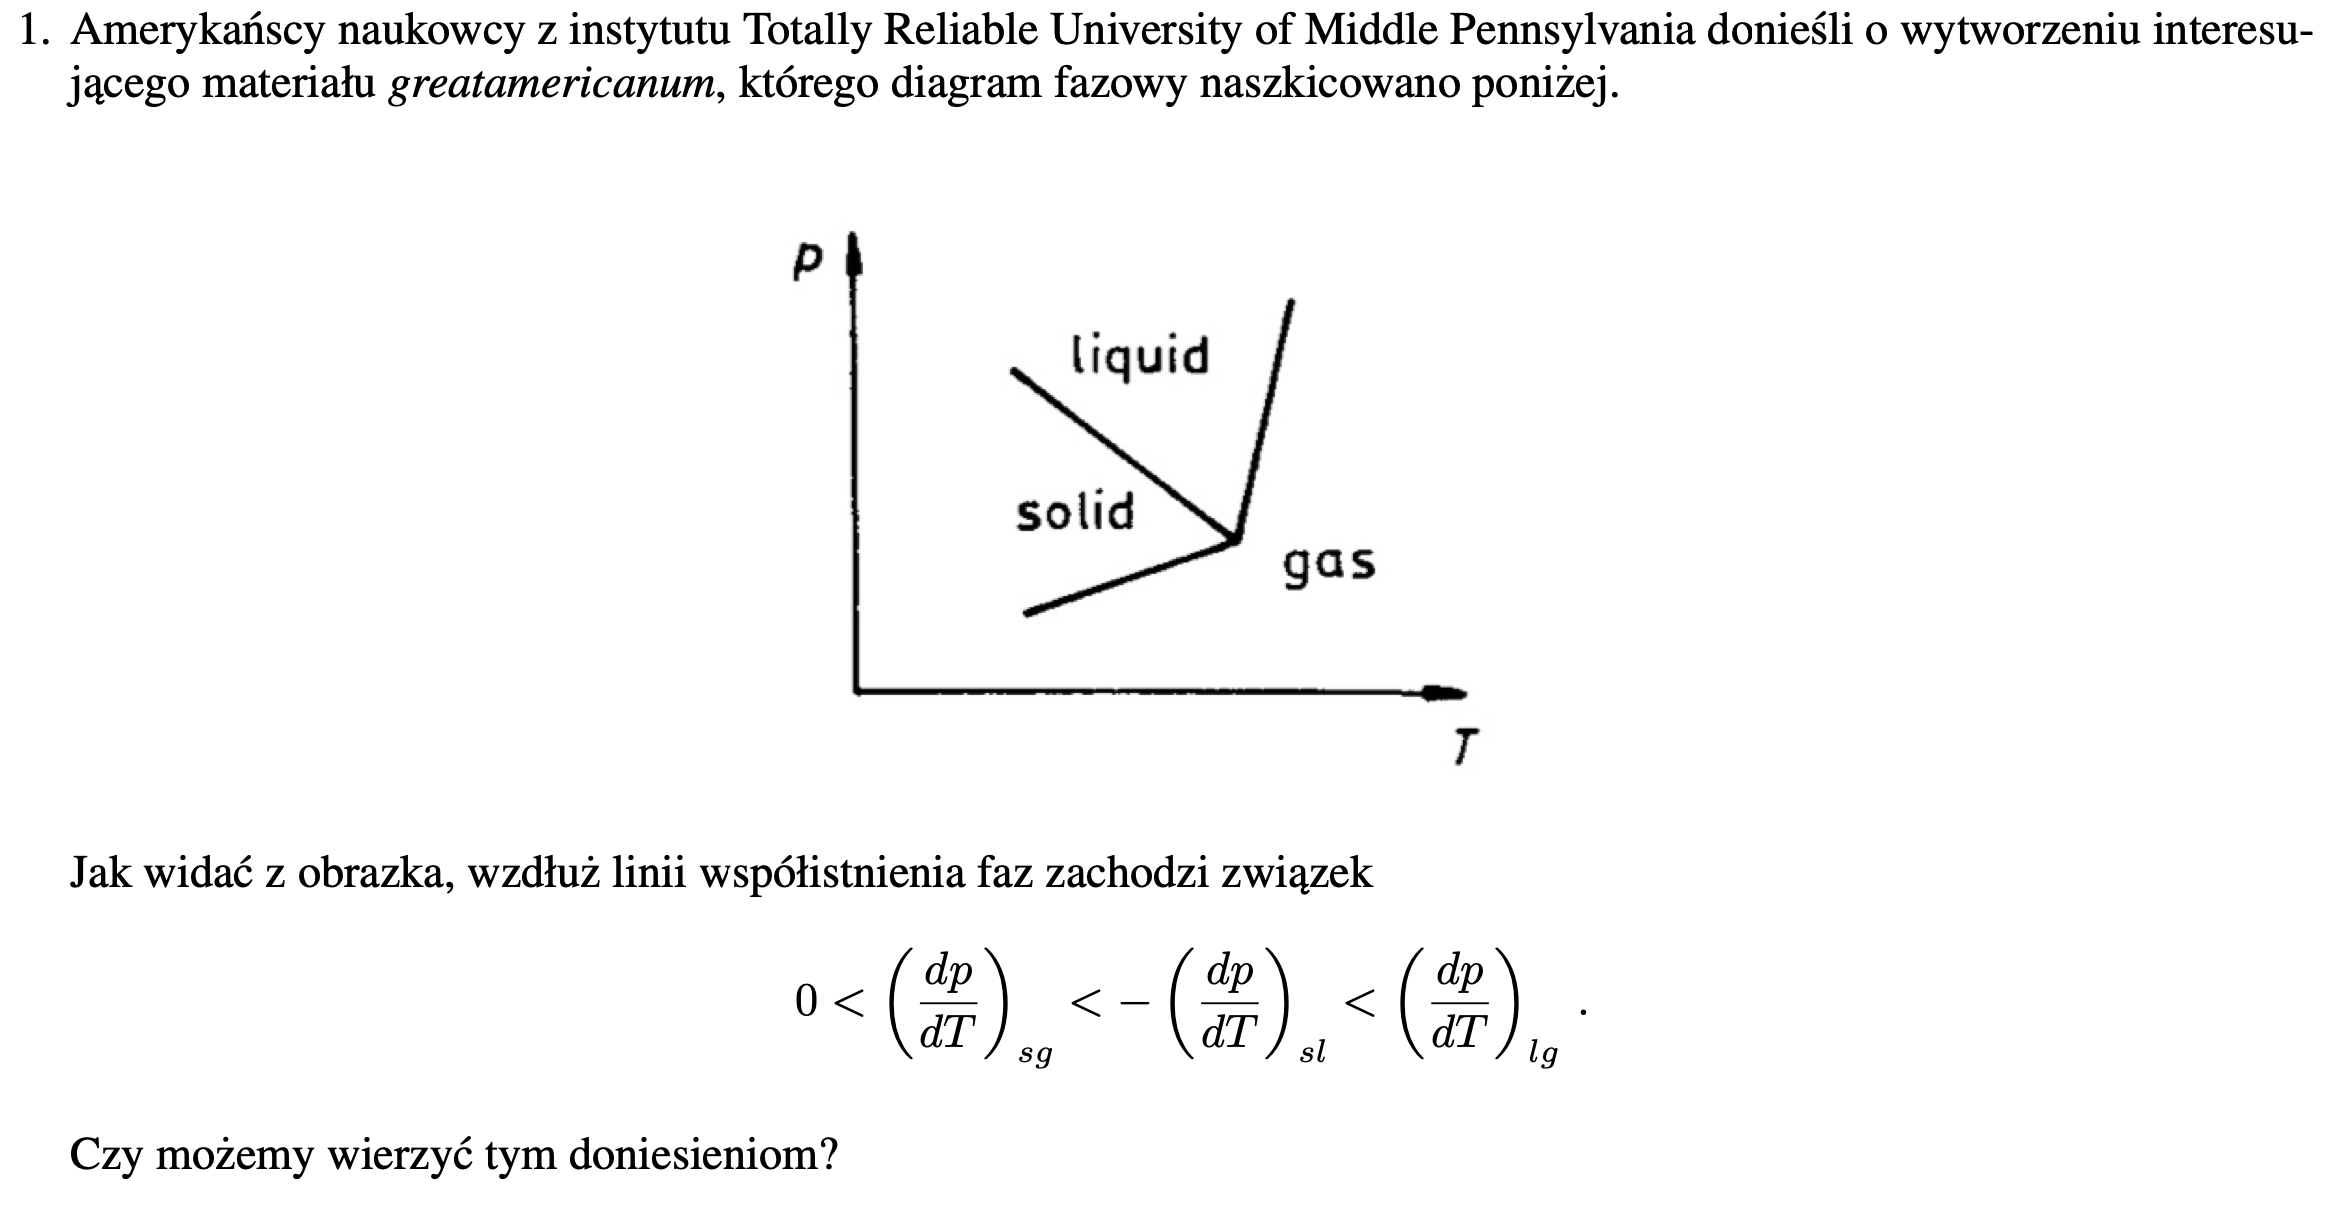
\includegraphics[width=\linewidth]{z1.png}
\end{figure}

\section{Rozwiązanie}

Wiadomo, że $\frac{\mathrm{d} p}{\mathrm{~d} T}$ można zapisać jako $\frac{Q}{T \Delta v}$, gdzie $Q$ to ciepło przemiany, $T$ to temperatura przemiany. Po dłuższym wpatrywaniu się w rysunek wywnioskować można, że ciepła każdej z przemian będą większe od 0. Podobnie temepratury przemiany będą większe od 0. Skoro, tak to na podstawie nierówności podanych w treści zadania wywnioskować można, że dla $\Delta v$ spełnione są nierówności:
$$
\begin{gathered}
\Delta v_{s g}>0 \\
\Delta v_{s l}<0 \\
\Delta v_{l g}>0
\end{gathered}
$$
Dla wygody wprowadźmy oznaczenia $A=\frac{Q_{s g}}{T_{s g}}, B=\frac{Q_{s l}}{T_{s l}}, C=\frac{Q_{l g}}{T_{l g}}$. Wówczas nierówności z treści zadania zapisać można jako:
$$
0<\frac{A}{\Delta v_{s g}}<-\frac{B}{\Delta v_{s l}}<\frac{C}{\Delta v_{l g}}
$$
Dostajemy stąd układ 3 nierówności, których prawdziwość chcemy sprawdzić.
$$
\begin{aligned}
\frac{A}{\Delta v_{s g}} &<-\frac{B}{\Delta v_{s l}} \\
\frac{A}{\Delta v_{s g}} &<\frac{C}{\Delta v_{l g}} \\
-\frac{B}{\Delta v_{s l}} &<\frac{C}{\Delta v_{l g}}
\end{aligned}
$$
Przekształćmy te nierówności:
$$
\begin{gathered}
A \Delta v_{s l}>-B \Delta v_{s g} \\
C \Delta v_{s g}>A \Delta v_{l g} \\
-B \Delta v_{l g}>C \Delta v_{s l}
\end{gathered}
$$
Dodając stronami 1 i 3 nierówność oraz 2 i 3 dostajemy nierówności:
$$
\begin{aligned}
&(A+B-C) \Delta v_{s l}>0 \\
&(A+B-C) \Delta v_{l g}<0
\end{aligned}
$$
Wynika z tego, że zachodzi $A+B-C<0$. Dodajmy teraz stronami 1 i 2 nierówność. Dostajemy z tego:
$$
\begin{gathered}
A\left(-\Delta v_{s l}+\Delta v_{l g}\right)<(B+C) \Delta v_{s g} \\
A\left(\Delta v_{s l}-\Delta v_{l g}\right)+(B+C) \Delta v_{s g}>0
\end{gathered}
$$
Ale wiemy, że $A<-B+C$, a stąd:
$$
(-B+C)\left(\Delta v_{s l}-\Delta v_{l g}\right)+(B+C) \Delta v_{s g}>A\left(\Delta v_{s l}-\Delta v_{l g}\right)+(B+C) \Delta v_{s g}>0
$$

$$
\begin{gathered}
2 B \Delta v_{l g}+2 C \Delta v_{s l}>0 \\
\frac{C}{\Delta v_{l g}}<-\frac{B}{\Delta v_{s l}}
\end{gathered}
$$
Co jest sprzeczne z początkowymi nierównościami. Wynika stąd, że taka substancja nie może istnieć.

\end{document}